\section*{\large{ВВЕДЕНИЕ}}

Цель лабораторной работы --- разработать программу шифровальной машины <<Энигма>> \cite{Enigma}.

Задачи лабораторной работы:

\begin{enumerate}
    \item провести анализ работы шифровальной машина <<Энигма>>;
    \item описать алгоритм шифрования;
    \item релизовать описанный алгоритм.
\end{enumerate}

\clearpage
\section{Аналитическая часть}

Шифровальная машина <<Энигма>> состоит из трех основных частей:
\begin{enumerate}
    \item роторы --- диски обладающие 26 гранями, где каждая грань представляла собой нумерацию английского алфавита;
    \item рефлектор --- статический механизм, позволящий машине также расшифровать текст;
    \item коммутатор --- набор парных шифров.
\end{enumerate}

\subsection{Алгоритм работы машины}

На вход <<Энигме>> подается строка, которая разбивается на символы. 
Далее символ проходит через коммутационную панель, который меняет символ в соотвествии с настройкой.
После прохождения панели, символ проходит черз три диска и попадает на рефлектор.
После работы рефлектора, символ отправляется обратно на диске и оканчательно шифруется через коммутатор.
Затем один ротор совершает оборот, если ротор обернулся 26 раз, то поворачивается следующий.


\clearpage

\section{Конструкторская часть}

\subsection{Разработка алгоритма}

На рисунке \ref{fig:alg} приведена схема работы шифровальной машины Энигма.


\begin{figure}[ht!]
	\centering
	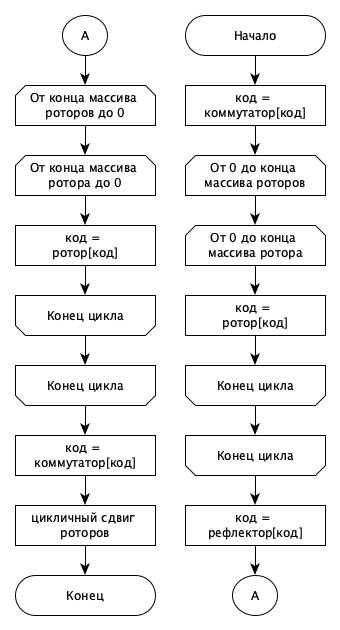
\includegraphics[width=0.6\linewidth]{assets/graphs/enigma-algo.png}
	\caption{Схема работы шифровальной машина Энигма}
	\label{fig:alg}
\end{figure}

\clearpage

\section{Технологическая часть}

\subsection{Средства реализации}

Для реализации ПО был выбран язык C++ \cite{c++}.
В данном языке есть все требующиеся инструменты для данной лабораторной работы.
В качестве среды разработки была выбрана среда VS code \cite{vscode}.

\subsection{Реализация алгоритма}

\begin{lstlisting}
uint8_t Enigma::encrypt(uint8_t code) {
    uint64_t rotor_queue = 1;
    uint8_t new_code = code;

    if (code > size_rotor) {
        throw std::out_of_range("Code bigger than size of rotor");
    }
    new_code = commutator[new_code];
    for (auto &rotor: rotors) {
        new_code = rotor[new_code];
    }
    new_code = reflector[new_code];
    for (int i = num_rotors - 1; i >= 0; --i) {
        try {
            new_code = find_rotor(i, new_code);
        }
        catch (const std::overflow_error& e) {
            std::cout << e.what() << std::endl;
        }
    }
    counter++;
    for (int i = 0; i < num_rotors; ++i) {
        if (counter % rotor_queue == 0) {
            rotor_shift(i);
        }
        rotor_queue *= size_rotor;
    }
    new_code = commutator[new_code];
    return new_code;
}
\end{lstlisting}


\subsection{Тестовые данные}

В таблице \ref{tbl:functional_test} приведены тесты для алгоритма шифрования Энигмы. 
Применена методология черного ящика. Тесты пройдены \textit{успешно}.



\begin{table}[ht!]
	\begin{center}
		\captionsetup{justification=raggedright,singlelinecheck=off}
		\caption{\label{tbl:functional_test} Функциональные тесты}
		\begin{tabular}{|c|c|c|}
			\hline
			Входная строка & Выходная строка \\ 
			\hline
			$ABOBA$ & $BCRGJ$\\
			$BCRGJ$  & $ABOBA$\\
			$<<>>$  & $<<>>$ \\
            $A$ & $T$\\
			$T$  & $A$\\
			\hline
		\end{tabular}
	\end{center}
\end{table}

\clearpage
\section*{\large{ЗАКЛЮЧЕНИЕ}}
В данной лабораторной работе:
\begin{enumerate}
    \item проведен анализ работы шифровальной машина <<Энигма>>;
    \item описан алгоритм шифрования;
    \item реализован описанный алгоритм;
\end{enumerate}